\documentclass[10pt]{article}

\usepackage[
  paperwidth=50mm,
  paperheight=180mm,
  margin=4mm
]{geometry}

\usepackage{amsmath}
\usepackage{amssymb}
\usepackage{multicol}
\usepackage{tikz}
\pagestyle{empty}

\begin{document}

\centering
{\Large\bfseries Mathematics Bookmark}

\vspace{3mm}
\hrule
\vspace{3mm}

\section*{Quadratic Equations}

Given

\[
ax^2 + bx + c = 0
\]

The roots are

\[
x=
\frac{-b\pm\sqrt{b^2-4ac}}
{2a}
\]

The discriminant is

\[
\Delta=b^2-4ac
\]

\begin{tabular}{ll}
$\Delta>0$ & two real roots\\
$\Delta=0$ & one repeated root\\
$\Delta<0$ & two complex roots
\end{tabular}

\vspace{4mm}
\hrule
\vspace{2mm}

\section*{Factoring}

Difference of squares

\[
a^2-b^2=(a-b)(a+b)
\]

Perfect squares

\[
(a+b)^2=a^2+2ab+b^2
\]

\[
(a-b)^2=a^2-2ab+b^2
\]

\vspace{4mm}
\hrule
\vspace{2mm}

\section*{Exponent Rules}

\[
a^m a^n=a^{m+n}
\]

\[
\frac{a^m}{a^n}=a^{m-n}
\]

\[
(a^m)^n=a^{mn}
\]

\[
(ab)^n=a^n b^n
\]

\[
a^{-n}=\frac1{a^n}
\]

\vspace{4mm}
\hrule
\vspace{2mm}

\section*{Logarithms}

\[
\log(ab)=\log a+\log b
\]

\[
\log\left(\frac ab\right)
=
\log a-\log b
\]

\[
\log(a^n)=n\log a
\]

\vfill

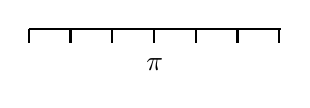
\begin{tikzpicture}
\draw[line width=0.8pt] (0,0) -- (3.2,0);
\foreach \x in {0,...,6}
  \draw[line width=0.8pt] (\x*0.53,0) -- ++(0,-0.18);
\node[below] at (1.6,-0.25) {$\pi$};
\end{tikzpicture}

\vspace{2mm}
{\small ``Mathematics is the art of explaining why.''}

\end{document}
